\section{Idea Progettuale}

\subsection{Ispirazione}

Visitando frequentemente questo luogo, che affascina per la presenza del lago, é stata notata la scarsità di bar o zone ristoro, pur essendoci spazi verdi attrezzati per \textit{Pic-Nic}. È stato pensato quindi di poter riconvertire il rimessaggio barche in un bar/chiosco (\cref{fig:stuttura}). Vista la sua collocazione é stato immaginato che il bar potesse offrire anche un servizio \textit{take-away} e cestini merenda da consumare in riva al lago. In questo modo si può compensare la quantità di tavoli disponibili, soprattutto nei periodi più ad alta affluenza. 

\begin{wrapfigure}[18]{r}{0.5\textwidth}
	\centering
	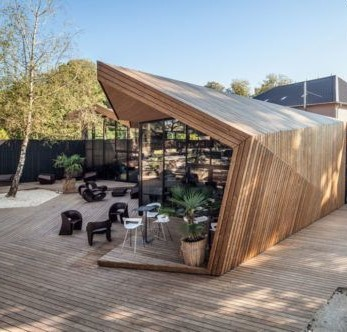
\includegraphics[width=0.4\textwidth]{image14}
	\caption{Struttura}
	\label{fig:stuttura}
\end{wrapfigure}

Trattandosi di una struttura semi aperta la quantità di tavoli disponibili è limitata; allo stesso tempo alcuni clienti potrebbero non essere propensi a dover consumare il pasto direttamente in loco in quanto sarebbero inclini ad utilizzare gli spazi verdi circostanti. Dare la possibilità del \textit{food-to-go} ci viene a vantaggio per 2 motivi, in primo luogo andiamo ad ampliare il bacino di utenti ed al contempo si possono servire più pasti non dovendosi preoccupare della quantità di tavoli disponibili; in secondo luogo il servizio \textit{take-away} porterebbe ad una riduzione totale del prezzo del servizio se questa modalità è scelta. In questo modo il cliente, che in caso di servizio al tavolo non avrebbe consumato, è invogliato sia dal prezzo minore che dal \say{vantaggio} di poter consumare in libertà. Lato commerciante questo servizio permette una riduzione dei costi di pulizia e, seppur in modo minore, del trattamento dei rifiuti.  Per questi motivi il servizio di \textit{take-away} potrebbe essere molto vantaggioso a livello commerciale.

L'obbiettivo è stato quello di realizzare una struttura  originale, che non fosse troppo statica e che non  stridesse con l’ambiente circostante . Non volevo un posto totalmente chiuso . Ho quindi individuato un progetto (\cref{fig:stuttura}) che,  con  le sue due  pareti libere,  permettesse di avere sempre la visione del lago e desse la sensazione di essere in uno spazio aperto. 

\clearpage
\subsection{Struttura}


La struttura, larga $4.30$ metri e lunga $5.40$ metri, è costruita con legno di larice come rivestimento(\cref{fig:listelli}), travi  d'acciaio \textit{IPE}  e chiusure trasparenti.

\begin{wrapfigure}[11]{r}{0.5\textwidth}
	\centering
	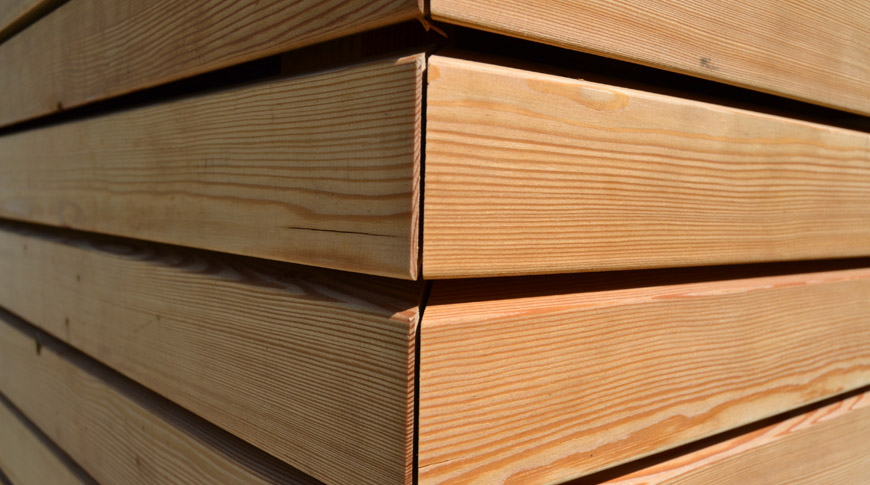
\includegraphics[width=0.4\textwidth]{image21}
	\caption{Listelli in legno}
	\label{fig:listelli}
\end{wrapfigure}

l legno di larice è un ottimo legno per rivestimenti per esterni, grazie alle sue notevoli proprietà isolanti. Il legno di larice tende ad assumere una tonalità grigiastra con il passare del tempo e tale escursione cromatica che lo rende particolarmente apprezzato . Inoltre ha una notevole durezza, resistenza alle sollecitazioni e un buon coefficiente di impermeabilità. 

Il lato nord è costituito da una parete di legno con due diverse inclinazioni; anche il lato ovest ,che si rivolge alla strada, è costituito da una parete di legno, mentre i lati est e sud sono aperti. Tutta la struttura poggia su una pedana di legno. I due lati aperti permettono il diretto accesso al bancone del bar e rendono la struttura integrata con l’ambiente che la circonda. 

La struttura è pensata per un uso estivo, visto che non offre tavoli al coperto. 
Ho previsto una chiusura dei lati aperti tramite una serranda orizzontale, 
in modo da chiudere il chiosco durante la notte o durante il periodo di non utilizzo. 

\begin{figure}[H]
	\centering
	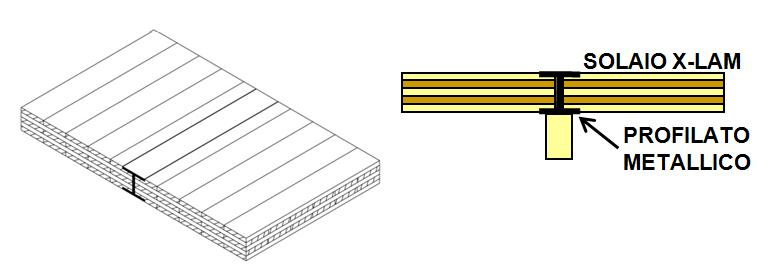
\includegraphics[width=0.8\textwidth]{image35}
	\caption{Interna struttura}
	\label{fig:pedana}
\end{figure}

\clearpage
La parte frontale della struttura si sviluppa a partire dalla forma di un pentagono, mentre la parte posteriore relativa ad un guscio di protezione. La scelta di di utilizzare un pentagono (\cref{fig:pentagono}) é stata pensata in modo da suddividere la struttura in due zone. Essa consente di avere una parte protettiva interna, come una chiocciola; allo stesso tempo il lato opposto presenta un apertura verso l'ambiente esterno.

\begin{figure}[H]
	\captionsetup[subfloat]{farskip=2pt,captionskip=8pt}
	\centering
	\subfloat[Vista laterale]{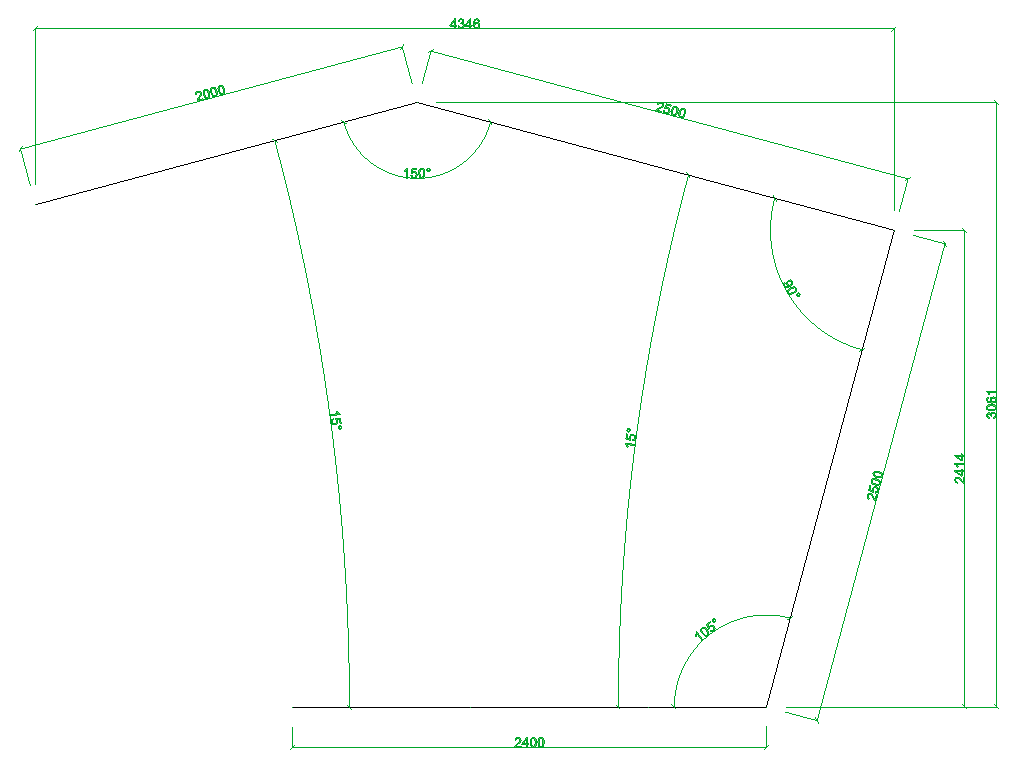
\includegraphics[width=6cm]{image43}}
	\hspace{1cm}
	\subfloat[Vista posteriore]{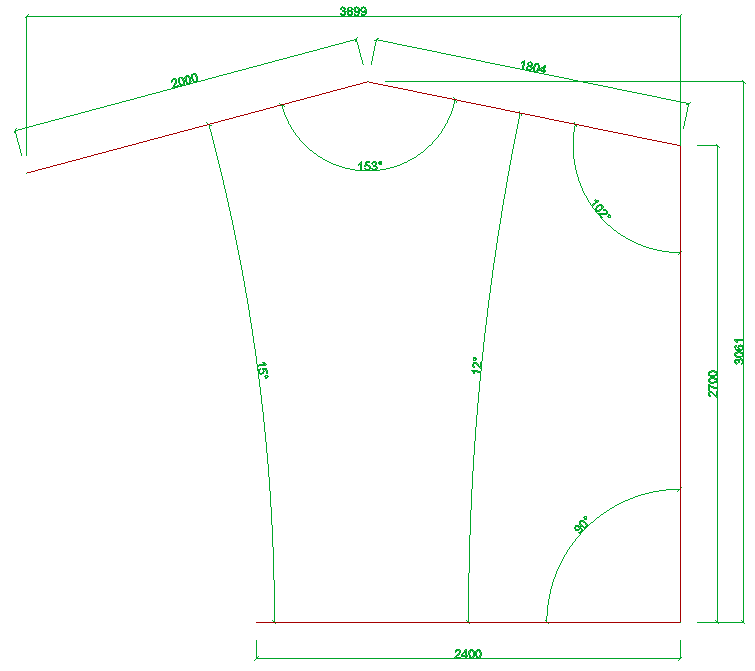
\includegraphics[width=6cm]{image1}}
\end{figure}

\begin{figure}[H]
	\captionsetup[subfloat]{farskip=2pt,captionskip=8pt}
	\centering
	\subfloat[Vista laterale: Guscio di protezione]{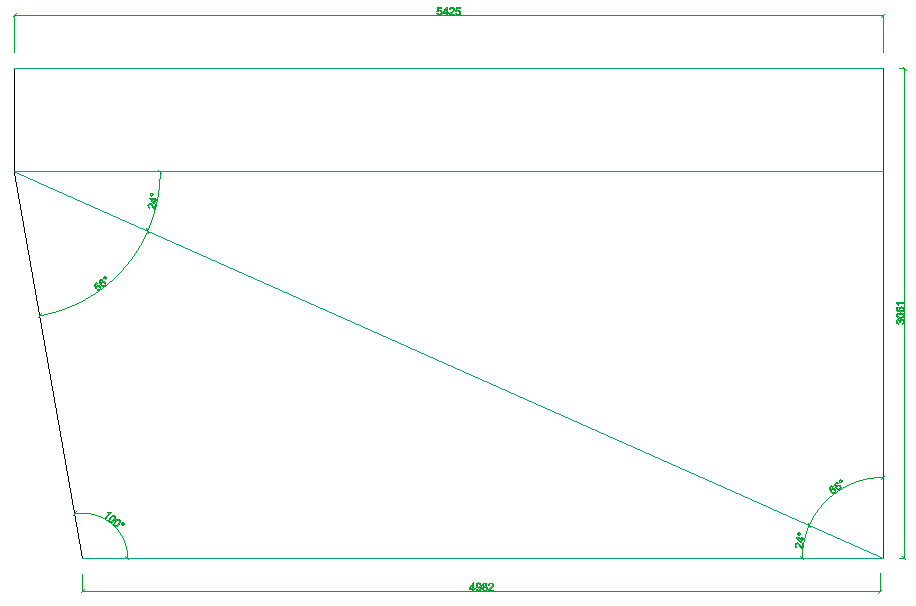
\includegraphics[width=6cm]{image34}}
	\hspace{1cm}
	\subfloat[Prospetto posteriore]{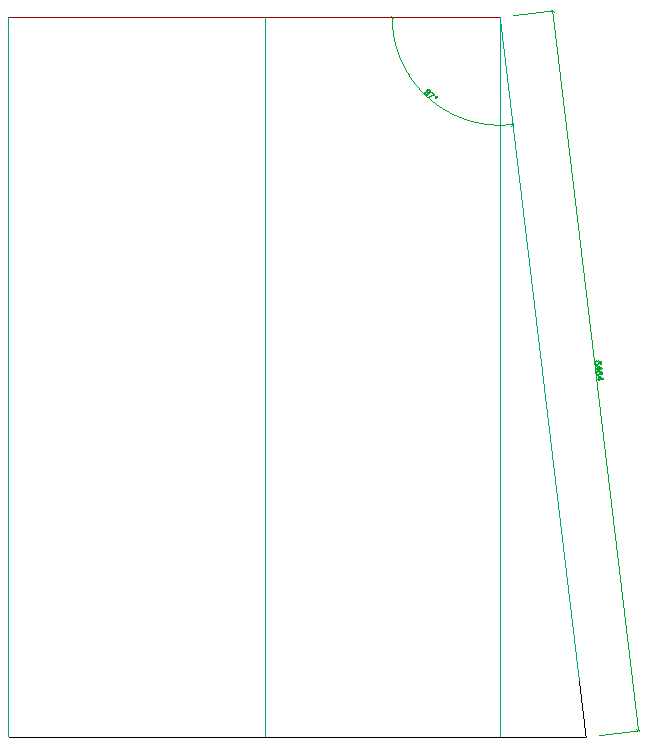
\includegraphics[width=6cm]{image32}}
	
	\caption{Viste}
	\label{fig:pentagono}
\end{figure}




\subsection{Analisi delle indicazione ergonomiche relative ai moduli costituenti il bancone da lavoro }

Il bar può essere suddiviso in quattro sotto-aree funzionali: piano di servizio, piano di lavoro, sotto banco  e retrobanco.

Il piano di servizio è posizionato poco più in alto rispetto a quello di lavoro. Può essere rivestito nel materiale che si preferisce, in linea con lo stile del locale. 
È l’elemento di comunicazione tra cliente e barista ed è l’area dove vengono servite le preparazioni e disposti gli snack per gli aperitivi. L'altezza totale del banco equivale all'altezza della bancalina, generalmente realizzata in marmo/pietra/corian o acciaio  ($\sim  1150mm$ da terra). In \cref{fig:persone} possiamo vedere una sezione del bancone in rapporto a due figure in modo da contestualizzare le misure.

\begin{figure}[H]
	\centering
	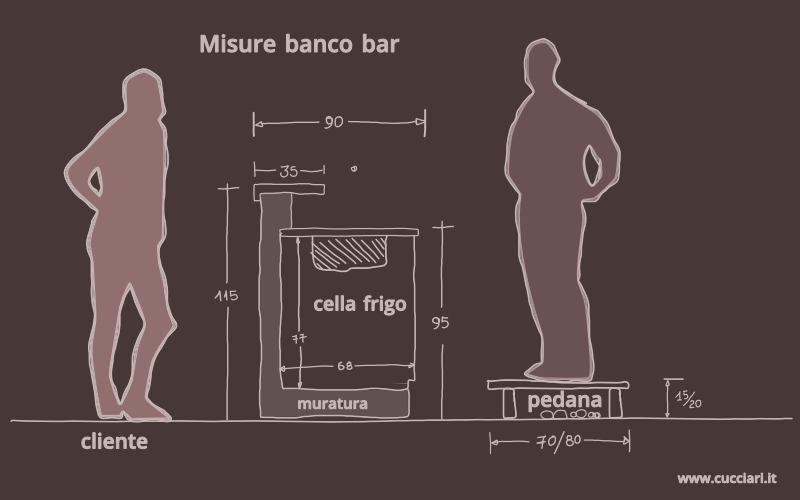
\includegraphics[width=0.6\textwidth]{image39}
	\caption{Banco bar con figure}
	\label{fig:persone}
\end{figure}

\noindent
Il piano di lavoro è la parte in cui vengono posizionate le attrezzature del bar utilizzate più spesso e meno ingombranti ed è appunto la zona in cui il barista prepara bevande e snack. L’altezza del piano di lavoro è di  $950mm$ da terra, in genere realizzato in acciaio inox. È qui che generalmente trova posto anche il lavello con acqua corrente e uno spazio per bottiglie di uso frequente.


Nel sottobanco trovano posto tutte quelle attrezzature più ingombranti, utilizzate quotidianamente e adibite soprattutto alla conservazione delle bevande e al lavaggio: tra questi il frigorifero, la macchina per il ghiaccio, la lavabicchieri o la lavastoviglie professionale. L'apertura dei vani refrigerati avviene attraverso sportelli o cassetti, interamente  in acciaio inox. Nel retrobanco del bar viene allestito il reparto caffetteria e espositore. Il retrobanco può essere neutro o refrigerato e composto da un numero variabile di armadietti con sportelli o cassetti, si possono dividere più o meno in due parti. Generalmente si distingue in due sezioni principali:


\begin{figure}[H]
	\captionsetup[subfloat]{farskip=2pt,captionskip=8pt}
	\centering
	\subfloat[Retro espositivo]{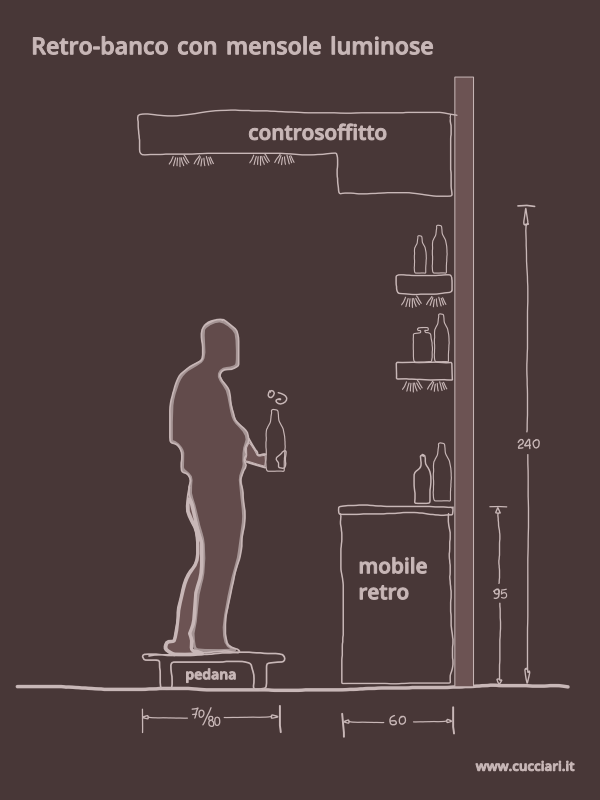
\includegraphics[width=6cm]{image46}}
	\hspace{1cm}
	\subfloat[Retro macchina caffè]{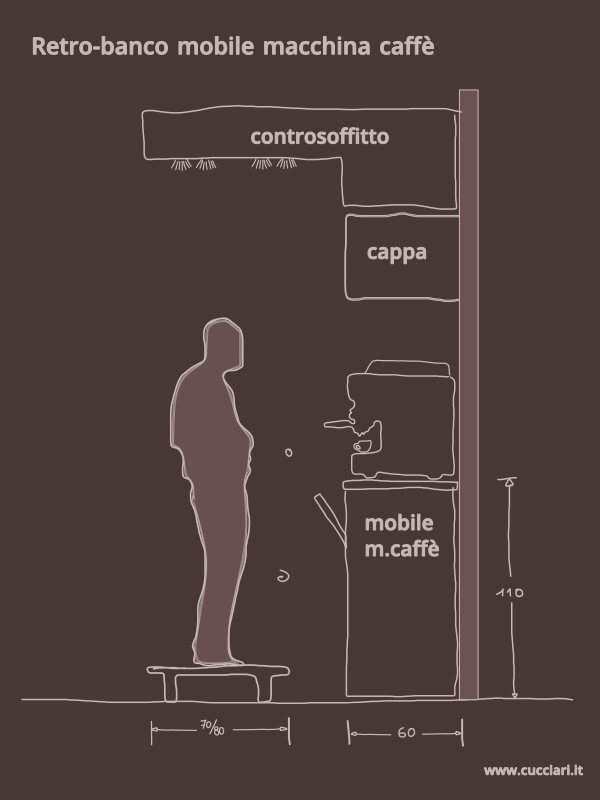
\includegraphics[width=6cm]{image8}}
	
	\caption{Retrobancone}
	\label{fig:imagesizes}
\end{figure}

\noindent
Retro multiuso e bottiglie.\todo{sistema} Composto da una base e da un'alzata su cui si applicano le mensole portabottiglie o i fondali attrezzati per vari servizi. Qui troviamo: cassetti, macina-caffè,  tramoggia per i fondi del caffè, spazzatura, uno spazio per la lavastoviglie oppure il produttore di ghiaccio, un vano per l’addolcitore ed infine la pompa macchina caffè.

